\section{Communication Interfaces}
\subsection{Begriffe}
Verschiedene Begriffe existieren im Zusammenhang mit Schnittstellen:
\begin{compactitem}
    \item \textbf{Synchron / Asynchron}: Synchrone Schnittstellen haben ein Taktsignal, welches signalisiert, wann Daten gültig sind. Asynchrone Schnittstellen brauchen dagegen kein Taktsignal. Synchronisation geschieht über einen Handshakingprozess.
    \item \textbf{Seriell / Parallel}: Daten werden seriell oder parallel (mit mehreren Signalleitungen gleichzeitig) übertragen.
    \item \textbf{On-Chip / Off-Chip Communication}: Kommunikation im Chip selbst wird oftmals parallel gelöst. Eine Kommunikation zwischen zwei verschiedenen Chips wird oft seriell implementiert.
\end{compactitem}

\subsection{Netzwerk Arten}
Verschiedene Netzwerk Arten existieren in der Praxis:
\begin{figure}[H]
    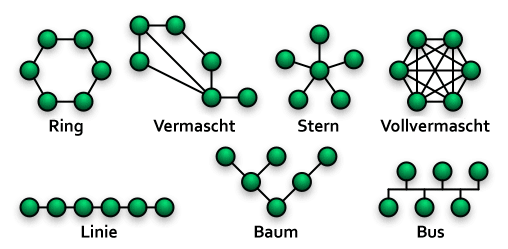
\includegraphics[width=0.5\textwidth]{images/netzwerkarten.png}
\end{figure}

\subsection{LVDS}
LVDS definiert kein Übertragungsprotokoll sondern eine Übertragungsart.
\begin{multicols}{2}
     \begin{figure}[H]
        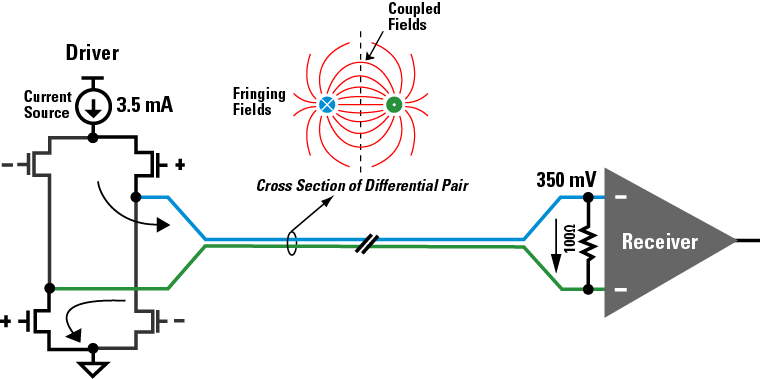
\includegraphics[width=0.5\textwidth]{images/lvds.png}
    \end{figure}

    \subsubsection{Prinzip}
    Die Signale werden anstelle mit einer Spannungsänderung mit einer Stromänderung übertragen. Das Signal schwingt somit nur um eine Spannung von $\pm$350mV.

    \subsubsection{Implementierung in VHDL}
    In VHDL kann LVDS nicht direkt synthetisiert werden. Der FPGA hat jedoch dennoch Pads, welche LVDS unterstützen. Diese müssen jedoch mithilfe von Constraints zugewiesen werden.
    \lstinputlisting[language=tcl]{code/tcl/lvds.xdc}
\end{multicols}

\subsection{VHDL Components}
\begin{multicols}{2}
Es gibt generische VHDL-Komponenten die für Kommunikationsinterfaces verwendet werden können. Sie alle beschreiben Teile des data link layers.
% \begin{itemize}
%   \item Schieberegister
%   \item RAM/ROM
%   \item FIFO Buffer
% \end{itemize}
\vfill\null
\columnbreak
\begin{figure}[H]
  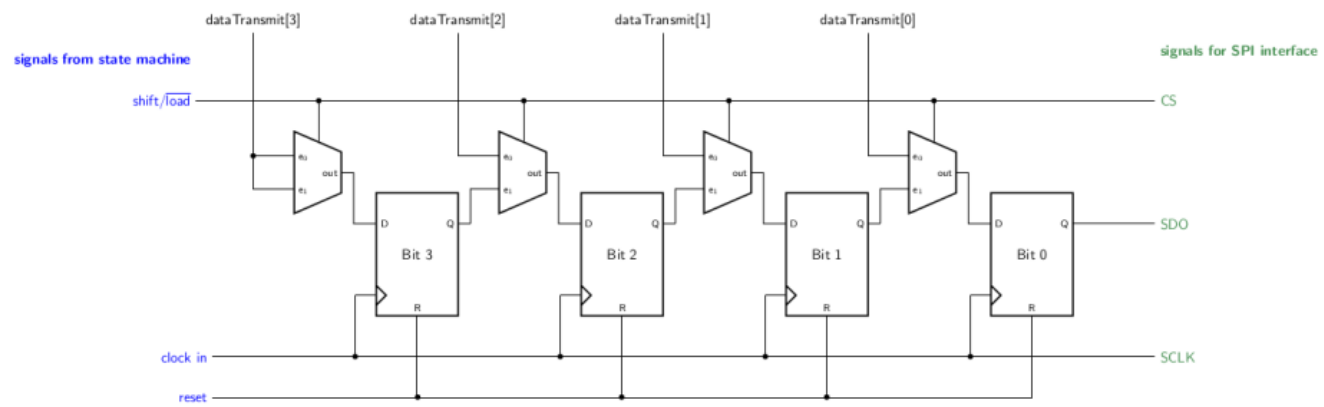
\includegraphics[width=0.5\textwidth]{images/shiftRegister.png}
\end{figure}
\end{multicols}
